% Options for packages loaded elsewhere
\PassOptionsToPackage{unicode}{hyperref}
\PassOptionsToPackage{hyphens}{url}
%
\documentclass[
]{article}
\usepackage{amsmath,amssymb}
\usepackage{lmodern}
\usepackage{ifxetex,ifluatex}
\ifnum 0\ifxetex 1\fi\ifluatex 1\fi=0 % if pdftex
  \usepackage[T1]{fontenc}
  \usepackage[utf8]{inputenc}
  \usepackage{textcomp} % provide euro and other symbols
\else % if luatex or xetex
  \usepackage{unicode-math}
  \defaultfontfeatures{Scale=MatchLowercase}
  \defaultfontfeatures[\rmfamily]{Ligatures=TeX,Scale=1}
\fi
% Use upquote if available, for straight quotes in verbatim environments
\IfFileExists{upquote.sty}{\usepackage{upquote}}{}
\IfFileExists{microtype.sty}{% use microtype if available
  \usepackage[]{microtype}
  \UseMicrotypeSet[protrusion]{basicmath} % disable protrusion for tt fonts
}{}
\makeatletter
\@ifundefined{KOMAClassName}{% if non-KOMA class
  \IfFileExists{parskip.sty}{%
    \usepackage{parskip}
  }{% else
    \setlength{\parindent}{0pt}
    \setlength{\parskip}{6pt plus 2pt minus 1pt}}
}{% if KOMA class
  \KOMAoptions{parskip=half}}
\makeatother
\usepackage{xcolor}
\IfFileExists{xurl.sty}{\usepackage{xurl}}{} % add URL line breaks if available
\IfFileExists{bookmark.sty}{\usepackage{bookmark}}{\usepackage{hyperref}}
\hypersetup{
  pdftitle={Integration of the model InVEST into the model EFForTS-ABM: new tool for dynamic simulation of socio-economic functions and biodiversity simultaneously},
  pdfauthor={Julia Henzler1*, Nils Beyer1, Sebastian Hanss1, Craig Eric Simpkins2, Jan Salecker3, Kerstin Wiegand1 (order have to be discussed)},
  hidelinks,
  pdfcreator={LaTeX via pandoc}}
\urlstyle{same} % disable monospaced font for URLs
\usepackage[margin=1in]{geometry}
\usepackage{color}
\usepackage{fancyvrb}
\newcommand{\VerbBar}{|}
\newcommand{\VERB}{\Verb[commandchars=\\\{\}]}
\DefineVerbatimEnvironment{Highlighting}{Verbatim}{commandchars=\\\{\}}
% Add ',fontsize=\small' for more characters per line
\usepackage{framed}
\definecolor{shadecolor}{RGB}{248,248,248}
\newenvironment{Shaded}{\begin{snugshade}}{\end{snugshade}}
\newcommand{\AlertTok}[1]{\textcolor[rgb]{0.94,0.16,0.16}{#1}}
\newcommand{\AnnotationTok}[1]{\textcolor[rgb]{0.56,0.35,0.01}{\textbf{\textit{#1}}}}
\newcommand{\AttributeTok}[1]{\textcolor[rgb]{0.77,0.63,0.00}{#1}}
\newcommand{\BaseNTok}[1]{\textcolor[rgb]{0.00,0.00,0.81}{#1}}
\newcommand{\BuiltInTok}[1]{#1}
\newcommand{\CharTok}[1]{\textcolor[rgb]{0.31,0.60,0.02}{#1}}
\newcommand{\CommentTok}[1]{\textcolor[rgb]{0.56,0.35,0.01}{\textit{#1}}}
\newcommand{\CommentVarTok}[1]{\textcolor[rgb]{0.56,0.35,0.01}{\textbf{\textit{#1}}}}
\newcommand{\ConstantTok}[1]{\textcolor[rgb]{0.00,0.00,0.00}{#1}}
\newcommand{\ControlFlowTok}[1]{\textcolor[rgb]{0.13,0.29,0.53}{\textbf{#1}}}
\newcommand{\DataTypeTok}[1]{\textcolor[rgb]{0.13,0.29,0.53}{#1}}
\newcommand{\DecValTok}[1]{\textcolor[rgb]{0.00,0.00,0.81}{#1}}
\newcommand{\DocumentationTok}[1]{\textcolor[rgb]{0.56,0.35,0.01}{\textbf{\textit{#1}}}}
\newcommand{\ErrorTok}[1]{\textcolor[rgb]{0.64,0.00,0.00}{\textbf{#1}}}
\newcommand{\ExtensionTok}[1]{#1}
\newcommand{\FloatTok}[1]{\textcolor[rgb]{0.00,0.00,0.81}{#1}}
\newcommand{\FunctionTok}[1]{\textcolor[rgb]{0.00,0.00,0.00}{#1}}
\newcommand{\ImportTok}[1]{#1}
\newcommand{\InformationTok}[1]{\textcolor[rgb]{0.56,0.35,0.01}{\textbf{\textit{#1}}}}
\newcommand{\KeywordTok}[1]{\textcolor[rgb]{0.13,0.29,0.53}{\textbf{#1}}}
\newcommand{\NormalTok}[1]{#1}
\newcommand{\OperatorTok}[1]{\textcolor[rgb]{0.81,0.36,0.00}{\textbf{#1}}}
\newcommand{\OtherTok}[1]{\textcolor[rgb]{0.56,0.35,0.01}{#1}}
\newcommand{\PreprocessorTok}[1]{\textcolor[rgb]{0.56,0.35,0.01}{\textit{#1}}}
\newcommand{\RegionMarkerTok}[1]{#1}
\newcommand{\SpecialCharTok}[1]{\textcolor[rgb]{0.00,0.00,0.00}{#1}}
\newcommand{\SpecialStringTok}[1]{\textcolor[rgb]{0.31,0.60,0.02}{#1}}
\newcommand{\StringTok}[1]{\textcolor[rgb]{0.31,0.60,0.02}{#1}}
\newcommand{\VariableTok}[1]{\textcolor[rgb]{0.00,0.00,0.00}{#1}}
\newcommand{\VerbatimStringTok}[1]{\textcolor[rgb]{0.31,0.60,0.02}{#1}}
\newcommand{\WarningTok}[1]{\textcolor[rgb]{0.56,0.35,0.01}{\textbf{\textit{#1}}}}
\usepackage{graphicx}
\makeatletter
\def\maxwidth{\ifdim\Gin@nat@width>\linewidth\linewidth\else\Gin@nat@width\fi}
\def\maxheight{\ifdim\Gin@nat@height>\textheight\textheight\else\Gin@nat@height\fi}
\makeatother
% Scale images if necessary, so that they will not overflow the page
% margins by default, and it is still possible to overwrite the defaults
% using explicit options in \includegraphics[width, height, ...]{}
\setkeys{Gin}{width=\maxwidth,height=\maxheight,keepaspectratio}
% Set default figure placement to htbp
\makeatletter
\def\fps@figure{htbp}
\makeatother
\setlength{\emergencystretch}{3em} % prevent overfull lines
\providecommand{\tightlist}{%
  \setlength{\itemsep}{0pt}\setlength{\parskip}{0pt}}
\setcounter{secnumdepth}{-\maxdimen} % remove section numbering
\usepackage{booktabs}
\usepackage{longtable}
\usepackage{array}
\usepackage{multirow}
\usepackage{wrapfig}
\usepackage{float}
\usepackage{colortbl}
\usepackage{pdflscape}
\usepackage{tabu}
\usepackage{threeparttable}
\usepackage{threeparttablex}
\usepackage[normalem]{ulem}
\usepackage{makecell}
\usepackage{xcolor}
\ifluatex
  \usepackage{selnolig}  % disable illegal ligatures
\fi
\newlength{\cslhangindent}
\setlength{\cslhangindent}{1.5em}
\newlength{\csllabelwidth}
\setlength{\csllabelwidth}{3em}
\newenvironment{CSLReferences}[2] % #1 hanging-ident, #2 entry spacing
 {% don't indent paragraphs
  \setlength{\parindent}{0pt}
  % turn on hanging indent if param 1 is 1
  \ifodd #1 \everypar{\setlength{\hangindent}{\cslhangindent}}\ignorespaces\fi
  % set entry spacing
  \ifnum #2 > 0
  \setlength{\parskip}{#2\baselineskip}
  \fi
 }%
 {}
\usepackage{calc}
\newcommand{\CSLBlock}[1]{#1\hfill\break}
\newcommand{\CSLLeftMargin}[1]{\parbox[t]{\csllabelwidth}{#1}}
\newcommand{\CSLRightInline}[1]{\parbox[t]{\linewidth - \csllabelwidth}{#1}\break}
\newcommand{\CSLIndent}[1]{\hspace{\cslhangindent}#1}

\title{Integration of the model InVEST into the model EFForTS-ABM: new
tool for dynamic simulation of socio-economic functions and biodiversity
simultaneously}
\author{Julia Henzler\textsuperscript{1}*, Nils
Beyer\textsuperscript{1}, Sebastian Hanss\textsuperscript{1}, Craig Eric
Simpkins\textsuperscript{2}, Jan Salecker\textsuperscript{3}, Kerstin
Wiegand\textsuperscript{1} (order have to be discussed)}
\date{4/28/2021}

\begin{document}
\maketitle

\hypertarget{methods}{%
\section{Methods}\label{methods}}

For the connection of socio-economic functions and biodiversity we
utilized two already existing models. For the economic part the dynamic
land-use change model EFForTS-ABM (Dislich et al. 2018) was used and for
the ecological part the static production function model
InVEST-Terrestrial Biodiversity (Kareiva et al. 2012, Version 3.9, Tier
1) was used. The initial landscapes for EFForTS-ABM are generated with
the landscape generator EFForTS-LGraf (Salecker et al. 2019). Landscapes
are comprised of regular grid cells of 100 x 100 cells, that is
25km\textsuperscript{2}. They represent a forested landscape in Sumatra
(Indonesia) with roads and villages of smallholder farming household
agents and agricultural fields (oilpalm and rubber) owned and farmed by
individual households. Households take rational land-use decisions with
the aim to maximize their economic benefit (Figure 1) (Fig.
\ref{fig:economic}). For further description of EFForTS-LGraf and
EFForTS-ABM see Salecker et al. (2019) and Dislich et al. (2018),
respectively. EFForTS-ABM was chosen as it is spatially-explicit and is
able to investigate how decisions of smallholders affect economic
(e.g.~household consumption) functions and landscape structure from
local to landscape scale and vice versa at various points in time.
EFForTS-ABM fits requirements for dynamically generate the input for
InVEST and dynamically process the output of InVEST.

\begin{figure}[h!]
  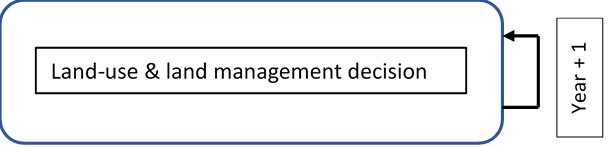
\includegraphics[width=0.5\textwidth]{"figures/png/Economic_simple.png"}
  \caption{Cumulative chronic mortality comparison. Black circles show empirical mortality values for a daily imidacloprid-dose of 0.01 ng/bee (taken from Suchail et al. (2001) Fig 2 Panel A), red circles show mortality values obtained from the approximation of as used in BEEHAVE-PESTICIDE.}
  \label{fig:economic}
\end{figure}

\begin{figure}
\centering
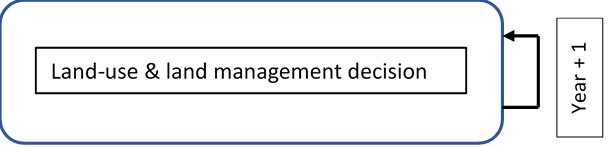
\includegraphics{figures/png/Economic_simple.png}
\caption{Figure 1: \textbf{EFForTS-ABM.} Yearly land-use and land
management decision of households.}
\end{figure}

Based on user-defined impacts to biodiversity, the terrestrial
biodiversity model of InVEST calculates a grid cell-level degradation
score for an user-defined Land-use and land-cover (LULC) map based on
location and distance of grid-cells to impacts. This degradation score
is than standardized to a grid-level habitat quality score (Figure 2).
The habitat quality score is used as a proxy for biodiversity based on a
simple habitat-analysis, which enables a rapid assessment of
biodiversity patterns. InVEST is a proven and widely applied software
tool for simulation of biodiversity and ecological functions. FOr
further information on the terrestrial biodiversity model InVEST see
(Sharp, R. et al., n.d.)

\begin{figure}
\centering
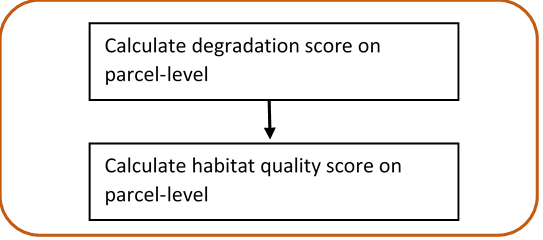
\includegraphics{figures/png/InVEST.png}
\caption{Figure 2: \textbf{InVEST-Terrestrial Biodiversity.} Calculation
of grid cell-level degradation and habitat quality score.}
\end{figure}

The realisation of the connection of both models was achieved by
Input-Output-Transfer. We mapped the output of EFForTS-ABM to input
InVEST and mapped the output InVEST to input EFForTS-ABM. First,
EFForTS-ABM generated the LULC-map and as many impact-maps as impacts
defined in tif-format and a corresponding sensitivity-table and
impact-table in csv-format. Second, InVEST generated the
habitat-degradation-map and habitat-quality-map in tif-format for
further processing in EFForTS-ABM (Figure 3). For transfering of maps,
we had to include an converter, as EFForTS-ABM can only use asc-format
and InVEST can only use tif-format.

\begin{figure}
\centering
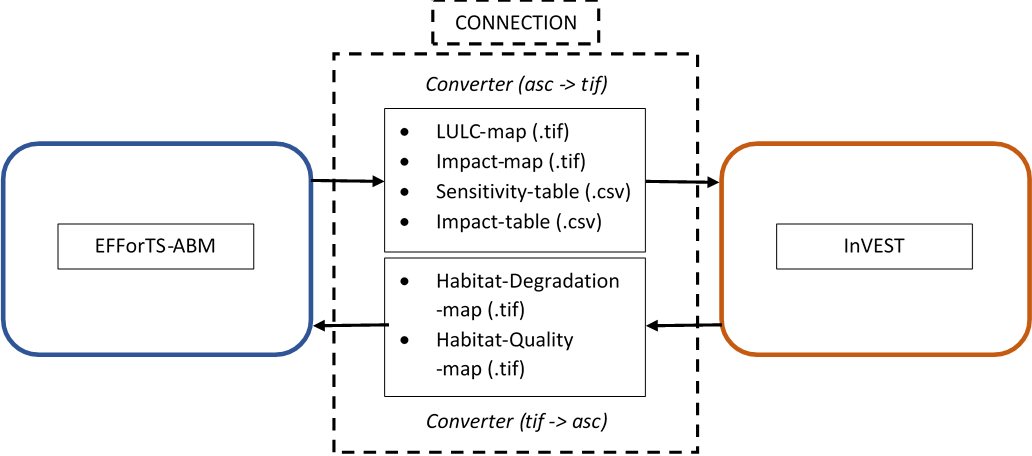
\includegraphics{figures/png/Input-Output-Transfer.png}
\caption{Figure 3: \textbf{Input-Output-Transfer between EFForTS-ABM and
InVEST}. The input of InVEST (LULC-map, Impact-map, Sensitivity-table,
Impact-table) are generated by EFForTS-ABM. The input of EFForTS-ABM
(Habitat-Degradation-map, Habitat-Quality-map) are generated by InVEST.}
\end{figure}

For evaluation of the connection between the dynamic land-use change
model EFForTS-ABM and the static production function model InVEST we
designed a requirement plan {[}citation?{]} divided into functional and
non-functional requirements. (Justification?) The functional
requirements include an testing scheme beginning at uni-tests to
integration-tests and ending with an acceptance-test {[}Citation?{]}.
Unit-tests were used to verify the correct implementation of functions.
This was realized by an isolated unit-testing modul within the model
EFForTS-ABM. It comprised each particular function implemented by the
connection of EfforTS-ABM and InVEST. We compared the simulated output
of each particular function separately to their expected output.
Genauer?

Integration-tests were used to verify the correct connection between
EFForTS-ABM an InVEST, which is fulfilled by correct
Input-Output-Transfer. This test was realized by an isolated
integration-testing modul within the model EFForTS-ABM. For more
convenient comparison of results, we chose a simplified parameter
setting (see table x) with a binary approach for habitat-assignment and
sensitivity of LULC-types to impacts. For the same reasons two
simplified landscapes - forest-landscape and single-field-landscape were
generated. First, the simulated grid cell-level habitat quality scores
of the forest-landscape were compared to the expected output to verify
the correct calculation of habitat-quality scores. Second, the simulated
grid cell-level habitat-quality scores of the one-field-landscape were
compared to the expected output to verify the correct reduction of
habitat quality scores by the defined impacts.

\begin{Shaded}
\begin{Highlighting}[]
\FunctionTok{library}\NormalTok{(kableExtra)}
\end{Highlighting}
\end{Shaded}

\begin{verbatim}
## Warning: package 'kableExtra' was built under R version 4.0.5
\end{verbatim}

\begin{Shaded}
\begin{Highlighting}[]
\CommentTok{\#Create dataframe from txt file}
\NormalTok{sensitivity }\OtherTok{\textless{}{-}} \FunctionTok{read.table}\NormalTok{(}\StringTok{"C:}\SpecialCharTok{\textbackslash{}\textbackslash{}}\StringTok{Users}\SpecialCharTok{\textbackslash{}\textbackslash{}}\StringTok{JuliaHenzler}\SpecialCharTok{\textbackslash{}\textbackslash{}}\StringTok{Documents}\SpecialCharTok{\textbackslash{}\textbackslash{}}\StringTok{3\_EFForTS}\SpecialCharTok{\textbackslash{}\textbackslash{}}\StringTok{1\_Biodiversity\_Submodel}\SpecialCharTok{\textbackslash{}\textbackslash{}}\StringTok{InVEST}\SpecialCharTok{\textbackslash{}\textbackslash{}}\StringTok{03\_Parameters}\SpecialCharTok{\textbackslash{}\textbackslash{}}\StringTok{Testing\_Scheme}\SpecialCharTok{\textbackslash{}\textbackslash{}}\StringTok{sensitivitytable\_integrationtest.txt"}\NormalTok{, }\AttributeTok{header =} \ConstantTok{TRUE}\NormalTok{)}
\NormalTok{sens }\OtherTok{\textless{}{-}} \FunctionTok{data.frame}\NormalTok{(sensitivity)}

\CommentTok{\#Create awesome table}
\NormalTok{sens }\SpecialCharTok{\%\textgreater{}\%}
  \FunctionTok{kbl}\NormalTok{() }\SpecialCharTok{\%\textgreater{}\%}
  \FunctionTok{kable\_styling}\NormalTok{() }\SpecialCharTok{\%\textgreater{}\%}
  \FunctionTok{footnote}\NormalTok{(}\AttributeTok{general =} \StringTok{"Classification (LULC) and names (NAMES) of LULC{-}types and their correspoding habitat assignment (HABITAT) and sensitivities to defined impacts (L\_oilpalm, L{-}rubber). "}\NormalTok{,}
           \AttributeTok{general\_title =} \StringTok{"Sensitivity table: "}\NormalTok{, }\AttributeTok{number\_title =} \StringTok{"Type I: "}\NormalTok{,}
           \AttributeTok{footnote\_as\_chunk =}\NormalTok{ T, }\AttributeTok{title\_format =} \FunctionTok{c}\NormalTok{(}\StringTok{"bold"}\NormalTok{)}
\NormalTok{  )}
\end{Highlighting}
\end{Shaded}

\begin{table}
\centering
\begin{tabular}[t]{r|l|r|r|r}
\hline
LULC & NAME & HABITAT & L\_oilplam & L\_rubber\\
\hline
1 & village & 0 & 0 & 0\\
\hline
2 & oilpalm & 0 & 1 & 1\\
\hline
3 & rubber & 0 & 1 & 1\\
\hline
4 & forest & 1 & 1 & 1\\
\hline
\multicolumn{5}{l}{\rule{0pt}{1em}\textbf{Sensitivity table: } Classification (LULC) and names (NAMES) of LULC-types and their correspoding habitat assignment (HABITAT) and sensitivities to defined impacts (L\_oilpalm, L-rubber). }\\
\end{tabular}
\end{table}

The acceptance test for verifying the simultaneoulsy simulation
socio-economic functions and biodiversity includes a theoretical
application example. Parameter setting is shown in table x. All test
were executed with the R package nlrx {[}Citation{]}

The non-functional requirements were reproducibility. For execution of
the simulations on the server, we designed a docker-file which included
the correct version of InVEST with all its required dependencies.
R-Studio, EFForTS-ABM. For executing the simulations on a
high-performance-cluster, we designed a singularity container, which
duplicates the docker-file into a singularity-file on the cluster.

\hypertarget{references}{%
\section*{References}\label{references}}
\addcontentsline{toc}{section}{References}

\hypertarget{refs}{}
\begin{CSLReferences}{1}{0}
\leavevmode\hypertarget{ref-http:ux2fux2fzotero.orgux2fusersux2f7697927ux2fitemsux2fRJF5NE77}{}%
Dislich, Claudia, Elisabeth Hettig, Jan Salecker, Johannes Heinonen,
Jann Lay, Katrin M. Meyer, Kerstin Wiegand, and Suria Tarigan. 2018.
{``Land-Use Change in Oil Palm Dominated Tropical Landscapes---An
Agent-Based Model to Explore Ecological and Socio-Economic
Trade-Offs.''} Edited by Edward Webb. \emph{PLOS ONE} 13 (1): e0190506.
\url{https://doi.org/10.1371/journal.pone.0190506}.

\leavevmode\hypertarget{ref-http:ux2fux2fzotero.orgux2fusersux2f7697927ux2fitemsux2fRNEYQF22}{}%
Kareiva, Peter, Heather Tallis, Taylor H. Ricketts, Gretchen C. Daily,
and Stephen Polasky. 2012. \emph{Natural Capital. Theory and Practice of
Mapping Ecosystem Services.} Oxford University Press.

\leavevmode\hypertarget{ref-http:ux2fux2fzotero.orgux2fusersux2f7697927ux2fitemsux2fZAPLKXXA}{}%
Salecker, Jan, Claudia Dislich, Kerstin Wiegand, Katrin M. Meyer, and
Guy Pe´er. 2019. {``EFForTS-LGraf: A Landscape Generator for Creating
Smallholder-Driven Land-Use Mosaics.''} Edited by Stephen P. Aldrich.
\emph{PLOS ONE} 14 (9): e0222949.
\url{https://doi.org/10.1371/journal.pone.0222949}.

\leavevmode\hypertarget{ref-http:ux2fux2fzotero.orgux2fusersux2f7697927ux2fitemsux2fUFHIJGJ8}{}%
Sharp, R., Douglass, J., Wolny, S., Arkema, K., Bernhardt, J.,
Bierbower, W., Chaumont, N., et al. n.d. {``InVEST
3.9.0.post77+ug.g875ac02 User's Guide.''} The Natural Capital Project,
Stanford University, University of Minnesota, The Nature Conservancy,
and World Wildlife Fund.

\end{CSLReferences}

\end{document}
